\documentclass[a4paper, 12pt]{article}
\usepackage{graphicx}
\usepackage{enumitem}
\usepackage{mathtools}
\usepackage{hyperref}
\usepackage{caption}
\usepackage{subcaption}
\def\code#1{\texttt{#1}}
\def\f#1{Figure \ref{fig:#1}}
\begin{document}

\title{\vspace{4.0cm}Applied GPU Programming - Assignment IV\\
\large DD2360 HT20}
\author{Pontus Asp}
\date{\today}
\maketitle
\thispagestyle{empty}
\pagenumbering{roman}
\newpage

\clearpage
\pagenumbering{arabic}

% Write here ->
\section{Git repository}
I uploaded my git repository to GitHub. I use the same git repository for the entire course but the folder structure requested is still followed under the root folder. I also have 2 extra directories, one for this report and one where I have code from lectures. I also was not sure if Exercise 4 should have been separate or included in this report so I did both, the standalone Exercise\_4.pdf can be found under the ex\_4 folder.
\\\\
Here is the link to my git repository:\\
\url{https://github.com/pontusasp/kth-dd2360/tree/master/Assignment_4}

% List and explain your extensions to the basic template provided by the course.
\section{Exercise 1}
The first thing I did when extending the template was writing a \code{helloworld} kernel in the char array \code{mykernel}. The reason for why I wrote the kernel is probably pretty self explanatory, but why it is in a char array might be more confusing. The kernel is written in a string since it will (can) be compiled at runtime by OpenCL, so that the kernel is compiled to be able to be used on the devices on the host system. Therefore it is in a char array so that the source code can be passed to the OpenCL API to be compiled and set up.

After writing the kernel I started writing code in the \code{main} function between the comments specifying where to insert my code. The first thing I added here was a call to the \code{clCreateProgramWithSource} which I passed some arguments to, and the two most significant ones were my context and a pointer to my source code.

What happens next is that \code{clCreateProgramWithSource} loads the program source code and stores it in a program object, which also gets associated with the OpenCL context I gave it, and then returns it.
However the program is not ready to be used yet, so what I did next was calling \code{clBuildProgram} which I passed the program object to. This function will then compile (and link) my program and update my program object.

After this point you might think that your program is ready to be executed, but one more API call is needed. To be honest, I could not find information of why exactly this step is needed but I am assuming that \code{clBuildProgram} simply compiles my executable program and the next step I did, \code{clCreateKernel} will take this program and prepare it to be launched on my OpenCL device, and also tell OpenCL the starting point of my program.

Now when my program, or should I say kernel, is compiled and loaded we need to launch it on the device. When launching the kernel we need to specify the size of our working groups and the number of work items we want to use (on a GPU a work item is a thread). We do all this with \code{clEnqueueNDRangeKernel} which we also will give our command queue and kernel to, along with the number of work groups and items, and also in what dimension we want to compute with. In our case, we where expected to use three dimensions, and decide our own group and item sizes. I went with groups of dimension \code{1x1x1} and set my working items to 4 in all 3 axis, so \code{4x4x4}. This should yield a result of $4^3 = 64$ prints, which is it.

When running a kernel on OpenCL it is running asynchronously from our code so the next thing I did was call \code{clFinish} and give it our command queue. This function simply waits for OpenCL to finish all the commands that we have queued and then returns control to our code. We do this so that we will not exit our program before OpenCL is finished.

% Explain how you solved the issue when the ARRAY_SIZE is not a multiple of the block size. If you implemented timing in the code, vary ARRAY_SIZE from small to large, and explain how the execution time changes between GPU and CPU.
\section{Exercise 2}
In this exercise we implemented a SAXPY program in OpenCL, I also implemented the optional time measurements. I solved the issue of \code{ARRAY\_SIZE} (which in my code is called \code{VSIZE}, but I will be calling it \code{ARRAY\_SIZE} here for simplicity) potentially not being a multiple of the block size by first getting how many block sizes could cover the entire array and then multiplying this with the block size again to get a number that is equal to, or larger than the \code{ARRAY\_SIZE}, that will be divisible by \code{BLOCK\_SIZE}. Here is the formula: $\frac{ARRAY\_SIZE + BLOCK\_SIZE - 1}{BLOCK\_SIZE} \cdot BLOCK\_SIZE$. Take into account that this works thanks to integer division, which gets rid of all decimals after the first division.

Since the device I use with OpenCL is a GPU, this is what I will reference the OpenCL device as. When comparing the execution time on the CPU vs the GPU with varying array sizes I found something interesting on this particular exercise. The total performance did not vary much with GPU vs CPU. When looking closer I however found that the reason was that by a large majority the time spent on the GPU was transferring data to and from the device memory. When measuring time a bit more in-depth I could see that the actual kernel execution by far outperformed the CPU execution on big array sizes. On small array sizes the kernel did however not do as well as the CPU, and also considering that the GPU has the penalty of memory transfer it was much slower than the CPU variant on small sizes. On very large arrays the GPU variant did start outperforming the CPU version but to my surprise not by much.

Here is a partial output from one run with an array size of $80 000 000$ (80M) and one run with the size of $10000$ (10k):

\subsection{80M Run:}
\begin{verbatim}
Computing SAXPY on the GPU...
    Computation done in   4.487000 ms
    Memory transfer:
        To Device:        55.451000 ms
        From Device:      87.244000 ms
    Total time:           147.182000 ms

Computing SAXPY on the CPU...
    Computation done in   155.476000 ms
\end{verbatim}

\subsection{10k Run:}
\begin{verbatim}
Computing SAXPY on the GPU...
    Computation done in   0.014000 ms
    Memory transfer:
        To Device:        0.121000 ms
        From Device:      0.022000 ms
    Total time:           0.157000 ms

Computing SAXPY on the CPU...
    Computation done in   0.019000 ms
\end{verbatim}

% 1. Measure the execution time of the CPU version, varying the number of particles.
%
% 2. Measure the execution time of the GPU version, varying the number of particles, like in 1).
%   2.1. Include data copying time to and from in the measurement.
%   2.2. For each GPU particle configuration, vary the block size in the GPU version from 16, 32, …, up to 256 threads per block.
%
% 3. Generate one or more performance figures based on your measurements in 1 and 2. Include it in the report with a description of the experimental setup (e.g., GPU used) and the observations obtained from the results. Explain how the execution time of the two version changes when the number of particles increases. Which block size configuration is optimal?
%
\section{Bonus Exercise 3}
\begin{figure}
    \centering
    \begin{subfigure}{.8\textwidth}
        \centering
        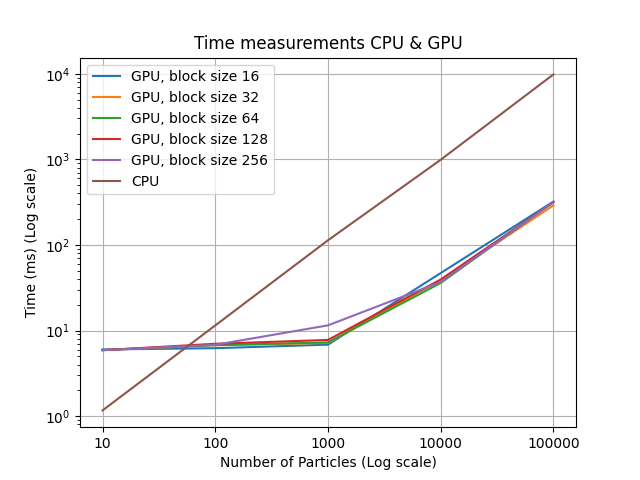
\includegraphics[width=1\linewidth]{ex_3_benchmark/ex_3.png}
        \caption{Benchmark GPU \& CPU}
        \label{fig:bench_3_both}
    \end{subfigure}
  \begin{subfigure}{.8\textwidth}
    \centering
    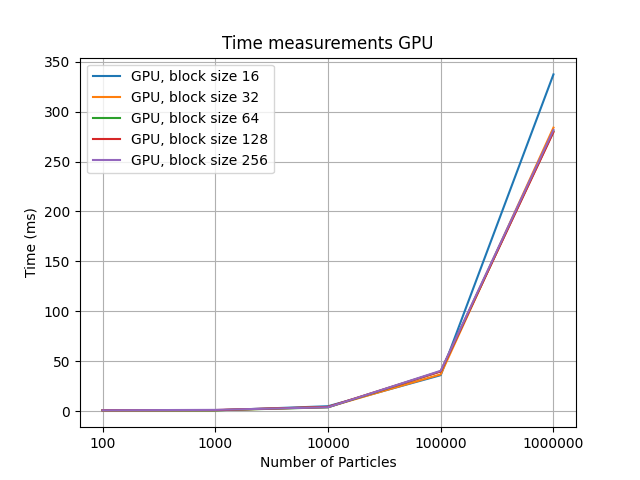
\includegraphics[width=1\linewidth]{ex_3_benchmark/ex_3_gpu.png}
    \caption{Benchmark only GPU}
    \label{fig:bench_3_gpu}
\end{subfigure}
\caption{Graphs showcasing the time measurements of a simulation with 10000 timesteps with varying block size, particles and GPU vs CPU. Benchmark done in Ubuntu 20.04 using a Nvidia GeForce GTX 1070 and an Intel(R) Core(TM) i7-9700K CPU @ 3.60GHz.}
\label{fig:bench_3}
\end{figure}
% 3. Describe the observations obtained from the results. Explain how the execution time of the two version changes when the number of particles increases. Which block size configuration is optimal?
%
% 4. Currently, the particle mover is completely offloaded to the GPU, only with data transfer at the beginning and end of the simulation. If the simulation involves CPU dependent functions (i.e. particles need to be copied back and forth every time step), would your observation in 3) still holds? How would you expect the performance will change in terms of GPU execution? Make an educated guess by timing your kernels.
%
In the bonus exercise, exercise 3, we implemented a particle simulation similar to what we have done previously. The difference this time is that we implemented it using OpenCL instead of CUDA. I did some benchmarks which you can see in \f{bench_3}. From the results you can see that the CPU implementation was more efficient for very low amounts of particles but was overtaken by the OpenCL implementation at around 90 particles. The CPU implementations graph was pretty much just a straight line which is what I expected since the only measurement done on the CPU is on the actual computation, and the computation is growing linearly with the amount of particles. In the OpenCL implementation we can see that it starts off at a higher value on the lower end than the CPU implementation. This is mainly because of the delay when we transfer data to the GPU. Continuing we can see that until around 1000 particles the graph is barely growing, I suspect this has to do something with that my GPU has a max work group size of 1024. Of course, we are not actually using this big of a group size but I have a hypothesis that this might be the max number of work items (threads) that can be launched at once on my GPU, so after this point the rest of the particles are in a queue to be simulated. So therefore the graph changes after this point but is still faster than my CPU. Looking closely at the graph of the GPU measurements in \f{bench_3_gpu} having a block size of 16 is the most efficient at a low amount of particles, but at a higher amount of particles a block size of 32 seems to be more optimal. So I would actually say that having a block size of 32 is better in this scenario if the trend keeps going as we do longer simulations.

If the particle simulation had CPU dependent functions and we needed to transfer the data back and forth between simulations the graphs would drastically change. Since transferring memory is a huge delay when doing small calculations in the version we made the transfer would also grow with the number of simulations which it currently does not do. Right now I am doing 10000 timesteps, which would need 10000 data transfers which would slow down the OpenCL implementation a lot. So I do not think the previous observations would hold at all if this was the case. 

\newpage
% WRITE STANDALONE FILE FIRST
\section{Exercise 4}
I pasted my exercise here as well since I was not sure if it should have been in its own file or not, if the separate file is needed it can be downloaded from the git repository in the ex\_4 folder. Here is a direct link: \url{https://github.com/pontusasp/kth-dd2360/blob/master/Assignment_4/ex_4/exercise_4.pdf}
% WRITE STANDALONE FILE FIRST
\subsection{Thoughts on OpenCL compared to CUDA}
When getting started with OpenCL it is easy to be overwhelmed by the amount of boilerplate code that needs to be written, and what function calls are needed for the setup etc. It is simply a steep learning curve to learn about for instance what contexts and command queues are, or about what the differences between devices and platforms, programs and kernels are. However the fact that OpenCL is so general and works on so many platforms is a very strong argument to using it. CUDA on the other hand, only works on Nvidia GPUs, and this could be both a good, and a bad thing. In my opinion, CUDA is much easier to get into, with less to remember than OpenCL, and with less boilerplate code. CUDA is also made specifically for GPUs, which is what makes it able to be a bit more simple than OpenCL since it has to take less platforms into account. With all this in mind, I do prefer using CUDA, but will probably use OpenCL since it works on more platforms.

Another thing to also consider is the performance differences between CUDA and OpenCL. Of course, CUDA should be faster on a Nvidia GPU since it is Nvidia's own API to their drivers but the question is - in reality, does it make a difference? I tested this by running the two particle simulations we created since I made them both equivalent on the CUDA and OpenCL implementation. My results actually surprised me. The OpenCL performed better than my CUDA variant when using more iterations and particles. But on fewer elements and iterations my CUDA implementation took the lead. I think the CUDA variant however has more room for optimization and if done properly could beat OpenCL at the higher amounts of particles and iterations. 

% Write here <--

\end{document}



%\begin{figure}
%  \centering
%  \begin{subfigure}{.5\textwidth}
%    \centering
%    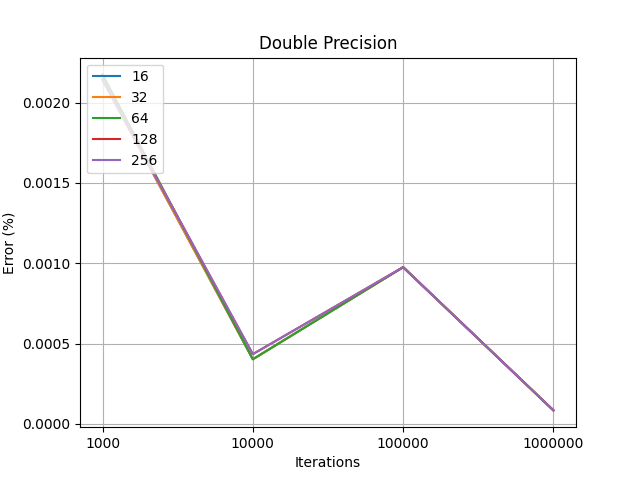
\includegraphics[width=1\linewidth]{graphs/ex_bonus_double_error.png}
%    \caption{Double Precision}
%    \label{fig:ex-single-double-error}
%  \end{subfigure}%
%  \begin{subfigure}{.5\textwidth}
%    \centering
%    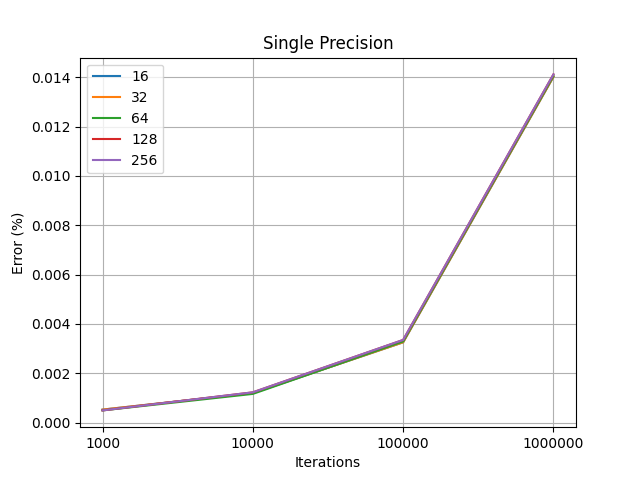
\includegraphics[width=1\linewidth]{graphs/ex_bonus_single_error.png}
%    \caption{Single Precision}
%    \label{fig:ex-bonus-single-error}
%  \end{subfigure}
%  \caption{Graphs of error using double and single precision with different amounts of iterations and block sizes.}
%  \label{fig:fig:ex-bonus-error}
%\end{figure}